\documentclass[preprint]{elsarticle}

\usepackage{amsmath,amssymb}
\usepackage[english]{babel}
\usepackage{listings}
\bibliographystyle{../styles/elsarticle-harv}

\newcommand{\oops}{\texttt{OOPS}}
\newcommand{\code}[1]{\ensuremath{\ulcorner#1\urcorner}}

% -*- latex -*-
% Definition of the Lua language for the listings package
% Time-stamp: <2008-11-30 15:27:16 rsmith>
% Written by Roland Smith <rsmith@xs4all.nl> and hereby placed in the public
% domain. 

\lstdefinelanguage{lua}
  {morekeywords={and,break,do,else,elseif,end,false,for,function,if,in,local,
     nil,not,or,repeat,return,then,true,until,while},
   morekeywords={[2]arg,assert,collectgarbage,dofile,error,_G,getfenv,
     getmetatable,ipairs,load,loadfile,loadstring,next,pairs,pcall,print,
     rawequal,rawget,rawset,select,setfenv,setmetatable,tonumber,tostring,
     type,unpack,_VERSION,xpcall},
   morekeywords={[2]coroutine.create,coroutine.resume,coroutine.running,
     coroutine.status,coroutine.wrap,coroutine.yield},
   morekeywords={[2]module,require,package.cpath,package.load,package.loaded,
     package.loaders,package.loadlib,package.path,package.preload,
     package.seeall},
   morekeywords={[2]string.byte,string.char,string.dump,string.find,
     string.format,string.gmatch,string.gsub,string.len,string.lower,
     string.match,string.rep,string.reverse,string.sub,string.upper},
   morekeywords={[2]table.concat,table.insert,table.maxn,table.remove,
   table.sort},
   morekeywords={[2]math.abs,math.acos,math.asin,math.atan,math.atan2,
     math.ceil,math.cos,math.cosh,math.deg,math.exp,math.floor,math.fmod,
     math.frexp,math.huge,math.ldexp,math.log,math.log10,math.max,math.min,
     math.modf,math.pi,math.pow,math.rad,math.random,math.randomseed,math.sin,
     math.sinh,math.sqrt,math.tan,math.tanh},
   morekeywords={[2]io.close,io.flush,io.input,io.lines,io.open,io.output,
     io.popen,io.read,io.tmpfile,io.type,io.write,file:close,file:flush,
     file:lines,file:read,file:seek,file:setvbuf,file:write},
   morekeywords={[2]os.clock,os.date,os.difftime,os.execute,os.exit,os.getenv,
     os.remove,os.rename,os.setlocale,os.time,os.tmpname},
   sensitive=true,
   morecomment=[l]{--},
   morecomment=[s]{--[[}{]]--},
   morestring=[b]",
   morestring=[d]'
  }


\lstset{language=lua, basicstyle=\small, stringstyle=\upshape,
stringstyle=\ttfamily, showstringspaces=false, tabsize=4}

\begin{document}

\begin{frontmatter}
\title{\oops: Title Here}

\author[gert]{Gert van Valkenhoef\corref{cor}}
\cortext[cor]{Corresponding author.}
\ead{g.h.m.van.valkenhoef@rug.nl}
\author[ai,tb]{Elske van der Vaart}
\ead{elskevdv@ai.rug.nl}
\author[ai]{Rineke Verbrugge}
\ead{rineke@ai.rug.nl}

\address[gert]{Department of Business and ICT, University of Groningen,\\
P.O. Box 800, 9700 AV, Groningen, The Netherlands}

\address[ai]{Department of Artificial Intelligence, University of Groningen,\\
P.O. Box 407, 9700 AK, Groningen, The Netherlands}

\address[tb]{Theoretical Biology Group, University of Groningen,\\
P.O. Box 14, 9750 AA, Haren, The Netherlands}

\begin{abstract}
abstract
\end{abstract}

\begin{keyword}
keyword1 \sep $\dots$ \sep keywordN
\end{keyword}

\end{frontmatter}

\section{Introduction}
\label{sec:introduction}

In this paper, we describe \oops, an {\it O}bject {\it O}riented {\it P}rover
for $S5_n$.
It is a tableaux-based theorem prover, specifically designed for use in a
classroom setting.
Although not as efficient as highly optimized provers like MSPASS
\citep{mspass2000} and FaCT \citep{fact1998}, or as flexible as highly
extensible provers like LoTReC \citep{lotrec2005} and the Tableau Workbench
\citep{twb2009}, we do think \oops\ offers a unique combination of features
that make it particularly suitable for educational purposes.

First, \oops\ offers support for $S5_n$, the logic typically used to model
human reasoning processes.
As far as we are aware, there are currently no other theorem provers which do
this.
Furthermore, \oops\ is capable of visualizing its tableaux proofs, and of
generating counterexamples to formulas that are false.
These two properties are very useful for educational proof tools, and they are
shared by at least two other systems: LoTReC can display its tableaux trees,
and the Logics Workbench \citep{heuerding1996} can print its derivations in
sequent calculi.

Another feature \oops\ has in common with LoTReC, as well as MSPASS, but with
few other theorem provers, is its free and convenient distribution.
\oops\ is packaged as a ZIP file that includes all dependencies, and once
extracted, can be run simply by double-clicking the resulting oops.jar file.
This is true for any operating system, provided the Java VM is available.
This in contrast to the Tableau Workbench, which must be built from source,
FaCT, which offers binaries only for Linux and Windows, and otherwise requires
Lisp, and the Logics Workbench, which is not open source, and can be difficult
or impossible to install, due to outdated dependencies.

A fifth property that makes \oops\ particularly attractive for educational use
is its graphic user interface.
Although simple, its GUI allows students to input formulas in an easy and
intuitive format, or to save and load files.
LoTReC, MSPASS and the the Logics Workbench also offer this functionality.

\oops' final educational attribute is its integrated scripting facility.
In our experience, most student projects involving theorem provers are efforts
to model riddles, or game situations.
This requires that students be able to build and extend theories, using loops
and conditionals where necessary.
Many proof tools, like the Logics Workbench, offer custom scripting languages
for this purpose.
\oops, by contrast, integrates the existing Lua\footnote{http://www.lua.org/}
scripting language.
Lua can be used to call most of \oops' functions, and offers an  rich input
language.
 
In the rest of this paper, we first offer a technical description of \oops,
including its proof system, its formal properties, its implementation in Java,
and the details of its input language (Section~\ref{sec:technical}).
This is followed by a more detailed description of \oops' educational
properties (Section~\ref{sec:features}), as well as a worked out example
(Section~\ref{sec:example}).
We conclude with a discussion of limitations and future work
(Section~\ref{sec:discussion}).


\section{Technical description}
\label{sec:technical}

In this section, we will first give a brief description of the tableau method
used in \oops\ and summarize the formal properties (soundness, completeness,
complexity) of the system. Then, we explain how the
tableau system is implemented in Java. Finally, we describe the input language
for modal formulas that is provided by \oops.

\subsection{\oops\ tableaux}
\label{sec:}

The \oops\ tableau system for $S5_n$ is a Java \citep{gosling2005}
implementation of the proof system {\bf ELtap} \citep{deboer2007,deboer2006}.  {\bf
ELtap}, in turn, draws on \citet{fitting1999} and \citet{beckert1997}.
\citet{halpern1992} provides a good review of tableau methods for modal logics.
Here, we summarize how tableaux are formalized in \oops. For a complete
description, see \citep{valkenhoef2008}.

When we construct a tableau, we do so with the aim of creating a Kripke model
in which a formula $\varphi$ is satisfied. This is done by assuming $\varphi$
is true and then systematically working out the implications of this
assumption. Specifically, \oops\ generates a collection of branches that each
represent alternative ways of working out these implications. A {\em branch}
$B$ consists of a number of nodes. A {\em node} $\gamma$ is a combination of a
{\em formula} $\psi$ and a {\em label} $\sigma$. A label is a systematically
chosen name for a world in the Kripke model that is being constructed. Branches
are created and 
expanded by the application of {\em rules} to existing nodes on
a branch. A {\em rule} $R$ consists of:

\begin{itemize}
\item A precondition $\mathrm{pre}(R)$, written above a horizontal bar, which
is a node containing variables;
\item A postcondition $\mathrm{post}(R)$, written below the horizontal bar,
which is a list of nodes containing variables. There are two types of
postconditions:
\begin{itemize}
\item Linear: add nodes to the current branch, written top-to-bottom;
\item Branching: create a number of new branches, written left-to-right, separated by a vertical bar.
\end{itemize}
\item Zero or more constraints, which restrict the values variables may take.
\end{itemize}
The rules employed by \oops\ are given in Table~\ref{tab:rules}. A rule $R$ is
applicable to a branch $B$, if there is a node $\gamma \in B$ that matches
$\mathrm{pre}(R)$, such that no constraints are violated and $R$ has not
previously been applied to $\gamma$.

In the case of modal rules, after the precondition $pre(R)$ has matched, we
may either need to create a new world (add a label part) or to match existing
worlds (labels). In the first case, we create a label part that is uniquely
identified, through a function $\code{\cdot}$ that encodes formulas as valid
label parts. In the latter case, the postcondition will contain a variable as
a placeholder for one of the label parts. Such a postcondition must be applied
to all labels that its label matches to.

A branch $B$ is {\em closed} if there is a label $\sigma$ and a formula
$\psi$, such that both $(\sigma, \psi) \in B$ and $(\sigma, \neg \psi)
\in B$. A branch $B$ is {\em open} if it is not closed and no more rules can be
applied to it. Thus, an open branch corresponds to a successful attempt to
satisfy $\varphi$, whereas a closed branch corresponds to a failed attempt to
satisfy $\varphi$. 
Specifically, for an open branch $B$, the labels determine the set of worlds
and the accessibility relations in the corresponding Kripke model. For each
label, the set of formulas given for that label determines the valuation in the
corresponding world in the Kripke model.
A tableau for $\varphi$ is closed if all branches are
closed, otherwise it is open. 

\begin{table}
\begin{center}

\renewcommand{\arraystretch}{1}
\begin{tabular}{ccc}

%% Double Negation Rule
\multirow{2}{*}{
	\begin{tabular} {c}
	{\it Double Negation}\\{\it Rule}
	\end{tabular}
}
&
	{\boldmath $\neg\neg$}
&
	%Third cell empty
\\ 
	% First cell empty
&
	\begin{tabular} {lc}
	$\sigma$&$\neg\neg\varphi$\\
	\hline
	$\sigma$&$\varphi$
	\end{tabular}
&
	%Third cell empty
\\[20pt]

%% Conjunctive Rules
\multirow{2}{*}{
	\begin{tabular} {c}
	{\it Conjunctive}\\{\it Rules}
	\end{tabular}
}
&
	{\boldmath $\wedge_\wedge$}
&
	{\boldmath $\wedge_\vee$}
\\
	% First cell empty
&
	\begin{tabular} {lc}
	$\sigma$&$\varphi\wedge\psi$\\
	\hline
	$\sigma$&$\varphi$\\
	$\sigma$&$\psi$
	\end{tabular}
&
	\begin{tabular} {lc}
	$\sigma$&$\neg(\varphi\vee\psi)$\\
	\hline
	$\sigma$&$\neg\varphi$\\
	$\sigma$&$\neg\psi$
	\end{tabular}
\\[20pt]

%% Disjunctive rules
\multirow{2}{*}{
	\begin{tabular} {c}
	{\it Disjunctive}\\{\it Rules}
	\end{tabular}
}
&
	{\boldmath $\vee_\wedge$}
&
	{\boldmath $\vee_\vee$} 
\\
	% First cell empty
&
	\begin{tabular} {lrlr}
	\multicolumn{4}{c}{$\sigma\;\;\;\;\neg(\varphi\wedge\psi)$}\\
	\hline
	$\sigma$&$\neg\varphi$&\multicolumn{1}{|r}{$\sigma$}&$\neg\psi$
	\end{tabular}
&
	\begin{tabular} {lrlr}
	\multicolumn{4}{c}{$\sigma\;\;\;\;\varphi\vee\psi$}\\
	\hline
	$\sigma$&$\varphi$&\multicolumn{1}{|r}{$\sigma$}&$\psi$
	\end{tabular}
\\[20pt]

%% Possibility Rules
\multirow{2}{*}{
	\begin{tabular} {c}
	{\it Possibility}\\{\it Rules}\\
	(where $i \neq j$)
	\end{tabular}
}
&
	{\boldmath $M_\Box$}
&
	{\boldmath $M_\Diamond$}
\\
	% First cell empty
&
	\begin{tabular} {lc}
	$\sigma.k_i$&$\neg \Box_j\varphi$\\
	\hline
	$\sigma.k_i.\code{\neg\varphi}_j$&$\neg\varphi$
	\end{tabular}
& 
	\begin{tabular} {lc}
	$\sigma.k_i$&$\Diamond_j\varphi$\\
	\hline
	$\sigma.k_i.\code{\varphi}_j$&$\varphi$
	\end{tabular}
\\[20pt]

%% Possibility Rules*
\multirow{2}{*}{
	\begin{tabular} {c}
	{\it Possibility} \\ {\it Rules$*$}
	\end{tabular}
}
&
	{\boldmath $M_\Box*$}
&
	{\boldmath $M_\Diamond*$}
\\
	% First cell empty
&
	\begin{tabular} {lc}
	$\sigma.k_i$&$\neg \Box_i\varphi$\\
	\hline
	$\sigma.\code{\neg\varphi}_i$&$\neg\varphi$
	\end{tabular}
&
	\begin{tabular} {lc}
	$\sigma.k_i$&$\Diamond_i\varphi$\\
	\hline
	$\sigma.\code{\varphi}_i$&$\varphi$
	\end{tabular}
\\[20pt]

% Basic Necessity Rules
\multirow{2}{*}{
	\begin{tabular} {c}
	{\it Basic Necessity}\\{\it Rules}\\
	(where $i \neq j$)
	\end{tabular}
}
&
	{\boldmath $K_\Box$}
&
	{\boldmath $K_\Diamond$}
\\
	% First cell empty
&
	\begin{tabular} {lc}
	$\sigma.k_i$&$\Box_j\varphi$\\
	\hline
	$\sigma.k_i.h_j$&$\varphi$
	\end{tabular}
& 
	\begin{tabular} {lc}
	$\sigma.k_i$&$\neg \Diamond_j\varphi$\\
	\hline
	$\sigma.k_i.h_j$&$\neg\varphi$
	\end{tabular}
\\[20pt]

% Basic Necessity Rules*
\multirow{2}{*}{
	\begin{tabular} {c}
	{\it Basic Necessity} \\ {\it Rules$*$}
	\end{tabular}
}
&
	{\boldmath $K_\Box*$}
&
	{\boldmath $K_\Diamond*$}
\\
	% First cell empty
& 
	\begin{tabular} {lc}
	$\sigma.k_i$&$\Box_i\varphi$\\
	\hline
	$\sigma.h_i$&$\varphi$
	\end{tabular}
&
	\begin{tabular} {lc}
	$\sigma.k_i$&$\neg \Diamond_i\varphi$\\
	\hline
	$\sigma.h_i$&$\neg\varphi$
	\end{tabular}
\\[20pt]

% Special Necessity Rules
\multirow{2}{*}{
	\begin{tabular} {c}
	{\it Special Necessity}\\{\it Rules}\\
	(where $i \neq j$)
	\end{tabular}
}
&
	{\boldmath $T_\Box$}
&
	{\boldmath $T_\Diamond$}
\\
	% First cell empty
& 
	\begin{tabular} {lc}
	$\sigma.k_i$&$\Box_j\varphi$\\
	\hline
	$\sigma.k_i$&$\varphi$
	\end{tabular}
& 
	\begin{tabular} {lc}
	$\sigma.k_i$&$\neg\Diamond_j\varphi$\\
	\hline
	$\sigma.k_i$&$\neg\varphi$
	\end{tabular}
\\[20pt]

% Special Necessity Rules*
\multirow{2}{*}{
	\begin{tabular} {c}
	{\it Special Necessity}\\{\it Rules$*$}
	\end{tabular}
}
&
	{\boldmath $R_\Box*$}
&
	{\boldmath $R_\Diamond*$}
\\
	% First cell empty
&
	\begin{tabular} {lc}
	$\sigma.k_i$&$\Box_i\varphi$\\
	\hline
	$\sigma$&$\varphi$
	\end{tabular}
&
	\begin{tabular} {lc}
	$\sigma.k_i$&$\neg\Diamond_i\varphi$\\
	\hline
	$\sigma$&$\neg\varphi$
	\end{tabular}
\\
\end{tabular}
\end{center}
\caption{Tableau Extension Rules (see Section~\ref{sec:implementation} for an explanation of how \oops\ applies these rules.)}\label{tab:rules}
\end{table}


Now, for any proof system, it is important that its proofs correspond exactly
to the semantics of the logic.
The proof system used by \oops\ has been shown to be both sound and complete
for $S5_n$ \citep{valkenhoef2008}. 
Furthermore, in the same work, the implementation
(Section~\ref{sec:implementation}) was
shown to correspond to the formal description of the proof method.
Unfortunately, this work also shows that the algorithm used by \oops\ needs exponential time in the worst case, whereas satisfiability for $S5_n$ is known to be {\sc pspace}-complete \citep{halpern1992}.
However, we believe that for educational purposes the functionality  offered
by \oops\ (see Section~\ref{sec:features}) easily makes up for this
shortcoming. Moreover, the implementation of these features does not depend on
the specific proof algorithm used. Thus, as future work, the current algorithm may
be replaced by one that is in {\sc pspace}.



\subsection{Implementation}
\label{sec:implementation}
In order to ensure the exhaustive, but non-redundant application of Table~\ref{tab:rules}'s rules,
\oops\ employs two data structures: the {\em match queue} and the {\em
necessities list}.
Whenever a node is added to the current branch, we attempt to match every
possible
rule to that node. The resulting matches are placed on the match queue. Now,
the Basic Necessity rules (Table~\ref{tab:rules}) pose a specific problem:
the postcondition may apply to labels that have not been generated yet. To
address this, partially matched postconditions of these rules are stored in
the necessities list. Whenever a new label is generated, any matches from this
list to the new label are added to the match queue.
These data structures are specific to a branch, i.e., when
a new branch is created, it receives a copy of the current match queue and
necessities list.

For reasons of efficiency,
the match queue is a priority queue and rules can be given a numeric
priority value, which specifies the order in which matches are applied to the
tableau. In this way, we may define a strategy to close branches as soon as
possible. For example, it is preferable to execute all possible non-branching
propositional rules before attempting to execute any other rules.

The rules are implemented in such a way that they are easily replaceable by a
different ruleset.
Moreover, the tableau generator allows the generation process to be monitored.
This enables the decoupled implementation of such features as tableau
visualization and counter-model construction (see Section~\ref{sec:features}).

\subsection{Input language}
\label{sec:language}

\oops\ employs an input language for formulas implemented using the SableCC
\citep{gagnon1998} compiler generator for Java. Propositions are input as
strings of characters and digits, starting with a lowercase character.  Agent
identities are represented by natural numbers. \oops\ uses the widely
understood infix notation for logical formulas. Table~\ref{tab:input} shows \oops\ ascii equivalents for different logical operators, as well as their precedences; lower numbers indicate stronger bindings.

\begin{table}
\centering
\begin{tabular}{lccccccc}
Connective & $\neg$ & $\wedge$ & $\vee$ & $\rightarrow$ &
$\leftrightarrow$ & $\Box_i$ & $\Diamond_i$ \\
\oops\ Symbol & \lstinline!~! & \lstinline!&! & \lstinline!|! & \lstinline!>!
& \lstinline!=! & \lstinline!#_i! & \lstinline!%_i! \\
Precedence & 1 & 2 & 3 & 4 & 4 & 1 & 1 \\
\end{tabular}
\caption{\oops\ Connectives.}
\label{tab:input}
\end{table}

In addition to this, the language allows the input of variables as
placeholders for either (sub-)formulas or agent identities. This is useful in
the definition of rules and allows one to create template formulas that can
be instantiated in different ways, by substitution.
Variables are strings of characters and digits that start with an uppercase
character.


\section{Functionality}
\label{sec:features}

For each feature:
\begin{itemize}
\item{Description}
\item{Implementation}
\item{Why is it useful?}
\item{Minimal example}
\end{itemize}

\subsection{Graphical User Interface}

\subsection{Integrated Scripting}

\subsection{Visualization of Tableaux}

\subsection{Visualization of Counter Models}

\subsection{Free and Convenient Distribution}

\begin{itemize}
\item Java runtime (run everywhere)
\item No installation: double-click JAR
\item Open Source
\end{itemize}

\subsection{Interchangeable Rule Sets}



\section{Example}
\label{sec:example}

To illustrate the educational potential of \oops\/, we present a worked-out example that models an exercise we have assigned to students of multi-agent systems in the past, at the Department of Artificial Intelligence at the University of Groningen.
We show how \oops' scripting can facilitate model construction and how its ability to visualize Kripke models can facilitate understanding of $S5_n$.
Our example concerns a simplified version of the `Wise Persons' puzzle:

\begin{quote}
There are two wise persons, Abelard (1) and Heloise (2). It is known to everyone that there are three hats: two red ones and one white one. The king puts a hat on the head of each of the two wise persons, who cannot see their own hat but can see the other person's hat (and they both know this). The king asks them sequentially if they know the color of the hat on their own head. The first person, Abelard, says that he does not know; the second person, Heloise, says that she knows.
Exercise: find out what must be the color of Heloise's hat.
\end{quote}

Let us define the propositions {\it r1} for `Abelard wears a red hat', {\it w1} for `Abelard wears the white hat', {\it r2} for `Heloise wears a red hat' and {\it w2} for `Heloise wears the white hat'.
In the full implementation of this example, available online,\footnote{\url{http://cloud.github.com/downloads/gertvv/oops/hats.lua}} a number of utility functions are given.
{\tt conj(f1, f2)} safely gives the conjunction of two formulas, {\tt knows(a1, f)} gives the formula $\square_{a1} f$' and {\tt knows2(a1, a2, f)} for $\square_{a1} \square_{a2} f$.
Finally, {\tt printAbelard(th)} and {\tt printHeloise(th)} give informative output on the knowledge states of Abelard and Heloise, given the theory th.

The initial situation can be modelled by simply defining the basic facts given in the puzzle and stating that both Abelard and Heloise are aware of these facts to sufficient depth.
Ofcourse, the background information should be common knowledge, but this is not accommodated in pure $S5_n$.
So we give knowledge to depth 2, the minimum level required to solve this puzzle.
The Lua code is as follows:
\begin{lstlisting}
-- each person has only one hat
oneHat = "(r1 = ~w1) & (r2 = ~w2)"

-- Abelard can see Heloise's hat
abelardSees = "#_1 w2 | #_1 r2"

-- Heloise can see Abelard's hat
heloiseSees = "#_2 w1 | #_2 r1"

-- background knowledge:
background = conj(conj(oneHat, oneWhite),
    conj(abelardSees, heloiseSees))

-- add the background and the wise persons'
-- knowledge about it (to depth 2)
th = oops.Theory()
th:add(background)
th:add(knows("1", background))
th:add(knows("2", background))
th:add(knows2("2", "1", background))
th:add(knows2("1", "2", background))
\end{lstlisting}
We can evaluate the agents' knowledge in the initial situation using the following statements:
\begin{lstlisting}
-- make sure we can show the counter model
oops.attachModelConstructor()

print("Initial Situation: ")
printAbelard(th)
printHeloise(th)
oops.showModel()
\end{lstlisting}
The counter model (generated by {\tt oops.showModel()}) to Heloise knowing the color of her hat is shown in Figure~\ref{fig:output1}. The console output is as follows:
\begin{verbatim}
Initial Situation:
Abelard doesn't know
Heloise doesn't know
\end{verbatim}

\begin{figure}
\centering
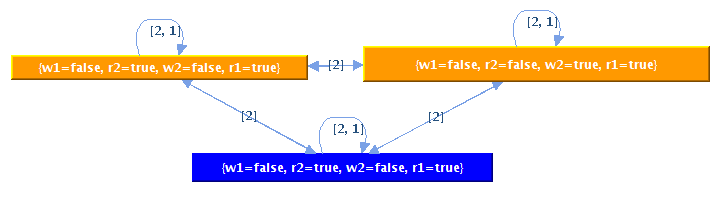
\includegraphics[width=0.4\textwidth]{images/demo04}
\caption{Counter model to Heloise knowing the color of her own hat in the initial situation of the `wise persons' puzzle. The counter model to Abelard knowing the color of his hat is almost identical, except that the relations between the worlds are for agent 1 (Abelard), not agent 2 (Heloise).}
\label{fig:output1}
\end{figure}

In the puzzle, Abelard is asked if he knows the color of his hat and responds that he doesn't. Heloise can now derive the color of her hat. We model this announcement by giving Heloise the knowledge that Abelard doesn't know the color of his hat.
\begin{lstlisting}
-- After Abelard announces he doesn't know:
abelardKnows = "#_1 w1 | #_1 r1"
th:add(oops.Formula("#_2 ~ F"):substitute(
    {F = abelardKnows}, {}))

print("After Abelard's announcement: ")
printAbelard(th)
oops.showModel()
printHeloise(th)
print("Consistent: " .. tostring(th:consistent()))
\end{lstlisting}
The output is as follows:
\begin{verbatim}
After Abelard's announcement:
Abelard doesn't know
Heloise knows his/her hat is red
Consistent: true
\end{verbatim}
Clearly, Abelard still doesn't know the color of his own hat (his own announcement doesn't help him), but Heloise is now aware that her hat is red, which is the correct solution to the puzzle.
The counter model generated by the above code is nearly the same as the one shown in Figure~\ref{fig:output1}, so it is not shown separately.

This example demonstrates the kind of assignment that can be designed with  \oops\/.
It gives students the experience of using a theorem prover, and lets them experiment with different assumptions, providing insight into the formal logic that underlies a familiar riddle.
This can all be done quickly and easily due to \oops's integrated scripting facility and GUI.


\section{Discussion}
\label{sec:discussion}

Discussion!

Future extensions:
\begin{itemize}
\item Rulesets in Lua
\item Simplification of theory/formula
\item Model checking, manipulation
\item stdin from GUI
\item {\sc pspace} prover
\item Comparison to/discussion of DEMO?
\end{itemize}


\bibliography{ref}

\end{document}
